\documentclass[
  a4paper,
  12pt,
  twoside,
  openright
]{report}

% ===== 日本語 =====
\usepackage{luatexja}

% ===== レイアウト =====
\usepackage[
  left=30mm,
  right=25mm,
  top=25mm,
  bottom=25mm
]{geometry}

% ===== 行間 =====
\usepackage{setspace}
\onehalfspacing

% ===== 段落制御（最重要） =====
\setlength{\parindent}{1\zw}
\setlength{\parskip}{0pt}

% セクション直後も字下げ
\usepackage{indentfirst}
\usepackage{caption}

% ===== 図挿入 =====
\usepackage{graphicx}
\usepackage{float}

% ===== 見出し番号 =====
\renewcommand{\chaptername}{第}
\renewcommand{\thechapter}{\arabic{chapter}}
\renewcommand{\thesection}{\thechapter.\arabic{section}}

% ===== 章見出しデザイン =====
\makeatletter
\renewcommand{\@makechapterhead}[1]{%
  \vspace*{50\p@}%
  {\parindent \z@ \raggedright
    \normalfont
    \Huge\bfseries 第\thechapter 章\quad #1\par\nobreak
    \vskip 40\p@
  }}
\makeatother

\begin{document}

% =====================
% 表紙（タイトルページ）
% =====================
\begin{titlepage}
  \thispagestyle{empty}

  \begin{center}
    \vspace*{20mm}

% ===== 年度＋ロゴ（文字は中央、ロゴは左）=====
\begin{center}
  % ロゴ（中央基準から左に配置）
  \makebox[0pt][r]{%
    \raisebox{-0.2ex}{%
      
\includegraphics[width=18mm]{fig/kindai.png}%
    }\hspace{10mm}%
  }%
  % 中央に来る文字
  {\LARGE 令和7年度\quad 卒業研究論文}
\end{center}

    \vspace{25mm}

    {\Huge\bfseries
      掌に付着するウイルス量の定量評価と\\
      洗浄による除去効率に関する研究
      \par}

    \vspace{35mm}

    {\Large
      92100104　上田 涼介\\
      92100124　岡本 悠椰\\
      92100108　川瀬 羽駈\\
      92005010　蔵岡 倫哉\\
      92000130　坪井 勇希\\
      92100113　寺地　翔\\
      92005035　森山 大史\\

      \par}

 % ===== フッター =====
    \vfill

    {\large 近畿大学工業高等専門学校 総合システム工学科 都市環境コース\\指導教員　安井 宣仁 准教授 \par}

    \end{center}
\end{titlepage}

% =====================
% 本文ページ番号の開始
% （表紙は番号なし → 第1章を 1 ページに）
% =====================
\cleardoublepage
\pagenumbering{arabic}
\setcounter{page}{1}

% ===== 本文 =====
% chap1.tex
\chapter{序論}

\section{研究背景 - 水系感染症の現状 -}

安全な飲料水や衛生設備が十分に整っていない地域では、細菌による水系感染症が多発している。
そのため、それらの地域では安全で清潔な水へのアクセスが非常に困難であり、
健康被害が深刻化している\textsuperscript{1)}
一方で、日本は水道の普及率が98.3\%と非常に高く\textsuperscript{2)}、
ほとんどの地域で清潔で安全な水を安定して利用することができる。
この点からも、日本は他国と比較して水資源の確保や衛生面で大きく進んでいることがわかる。

しかし、世界全体で見ると、いまだに多くの人々が安全で清潔な水を十分に利用できない状況にある。
汚染された水を飲用あるいは生活用水として使用することで感染症にかかる人が後を絶たず、
特に発展途上国では深刻な社会問題となっている。
代表的な水系感染症としては、コレラ、赤痢、チフス、A型肝炎などが挙げられ、
これらはいずれも汚れた水や不衛生な環境が主な原因で発生する。
世界保健機関（WHO）の報告\textsuperscript{3)}によると、
安全な飲料水を利用できない人は世界で約20億人以上にのぼり、
毎年、約505,000人が安全でない水および不十分な衛生環境を原因として死亡している。
従って、安全な水の確保は依然として世界的な課題である。

また、安全な水資源へのアクセスが困難となる要因として、
多くの発展途上国では水道管や浄水場といったインフラが十分に整備されていないことが挙げられる。
さらに、設備の老朽化や下水・工場排水の河川への直接流入によって水源が汚染される事例も多く、
こうした汚染は水系感染症の発生要因となり、健康面でも重大な影響を及ぼしている。

加えて、気候変動の影響による干ばつの増加や地下水の過剰利用によって、
利用可能な水資源そのものが減少している地域も存在する。
貧困により水道料金を支払えない、あるいは浄水設備を利用できない家庭も多く、
結果として不衛生な水に依存せざるを得ない状況が生じている。
紛争や政治的不安定によるインフラ破壊や資源管理の不全が重なる地域では、
状況はさらに深刻化する。

具体例として、2010年のハイチ大地震後には下水処理機能の喪失により汚染水が広がり、
大規模なコレラ流行が発生した。
また、内戦下のイエメンでは水道インフラの破壊と医療体制の崩壊により、
世界最大規模のコレラ流行が確認されている。
南アジアのスラム地域では上下水道未整備による飲料水汚染から赤痢が季節的に多発し、
難民キャンプにおいてもトイレ不足や水の共同利用による集団感染が報告されている。
これらはいずれも、災害・紛争・貧困・インフラ不足による衛生環境の悪化が
感染拡大の主要因となっている事例である。

日本においても、東日本大震災の際には水道が停止し、
手洗い用の水が不足したことで十分な手指衛生が困難となり、
ノロウイルスや感染性胃腸炎の集団発生が報告された。
このように、平時には安全とされる地域であっても、
災害時には水系感染症のリスクが急激に高まることが示されている。

%--------------------------------------------------

\section{既存研究の限界}

現在までに発表されている研究の多くは、
日常生活環境や医療現場など、比較的衛生状態が管理された状況を対象としており、
災害時や水道が利用できない状況、高度に汚染された水環境を想定した実験データは
十分に蓄積されていない。

人が日常生活の中でさまざまな物体に手で触れた際に、
どの程度の微生物が皮膚表面に付着するかを測定した研究はいくつか存在するが、
環境微生物の種類や濃度が大きく変化する災害時の状況に
そのまま適用することは困難である。
そのため、災害時を想定した実験的検討が求められている。

本節では、これまでに報告されている代表的な既存研究について概説する。

\paragraph{病院エレベーターの押しボタンと手指を対象とした菌の伝播に関する考察}\textsuperscript{4)}

松野 容子、水野 秀一、大徳 優子による研究では、
病院環境における菌の分布および動態を明らかにすることを目的として、
病棟エレベーターの押しボタンと手指を対象とした細菌学的検討が行われた。
使用人数別（1～8人）および経時間的（30～120分）に押しボタン上から検出された菌数は、
概ね0～300 CFUであり、その70\%以上が20 CFU未満であった。
一方で、最大1200 CFUが検出される事例も確認され、
一部の手指汚染状況によっては極めて高い汚染が生じ得ることが示された。

\paragraph{高度汚染した手指の衛生学的手洗いの検討}\textsuperscript{5)}

矢野 久子、小林 寛伊、奥住 捷子は、
高度に手指が汚染された状況を想定し、
手洗い時間や手洗い方法の違いによる除菌効果について検討を行った。
本研究では、病院現場における手洗い頻度や時間の短さが課題であることが指摘されている。

\paragraph{手洗い効果の細菌学的考察}\textsuperscript{6)}

石田 和夫、三浦 英雄は、
1997～1999年に学生399人を対象として、
水洗い、石鹸、消毒薬など複数の方法による手洗い前後の
手指生菌数を比較し、手洗い方法による除菌効果の違いを明らかにした。

\paragraph{高齢者介護施設における入居者の手指衛生の実態}\textsuperscript{7)}

中村 明世、岡田 淳子、飯田 忠行は、
高齢者介護施設における入居者の手指衛生の実態を調査し、
活動状況に応じて手指衛生方法や実施頻度が異なることを報告している。

%--------------------------------------------------

\section{本研究の目的と重要性}

災害発生時や安全な水資源へのアクセスが制限された状況では、
衛生環境が急激に悪化し、感染症リスクが著しく増大する。
しかし、このような特殊な状況を対象とした微生物学的研究は、
現時点では十分に行われていない。

特に災害時には、手洗いに使用できる清潔な水の確保が困難となるため、
通常時と比較して手指衛生の効果が低下する可能性がある。
また、現在の防災マニュアルにおいても、
使用する水の種類や量によってどの程度微生物が除去されるのかといった
科学的根拠は十分に示されていない。

そこで本研究では、災害時に水道などの安全な水源の利用が困難となり、
河川水、雨水、貯留水などの代替水源を使用する状況を想定し、
水を媒介とした水系感染症のリスク評価を行うことを目的とする。
具体的には、以下の事項について検討を行った。

\begin{itemize}
  \item 模擬水を用いた掌への水分付着量の定量化
  \item 大腸菌ファージを指標微生物として用いた掌への移行率評価
  \item 手洗い後の掌への微生物残存率の評価
  \item 統計解析および定量的微生物リスク評価（QMRA）の実施
\end{itemize}

得られた結果をもとに、災害時における感染症発生リスクを評価し、
安全な水資源へのアクセスが制限される状況においても実践可能な
効果的な手指衛生方法および感染症予防対策を提案することを
本研究の最終的な目的とする。

%--------------------------------------------------

\section{論文構成}

本論文は以下の構成からなる。

本研究は、災害時など安全な水資源が十分に確保できない状況において、
手指を介した水系感染症のリスクを定量的に評価することを目的として
実施された。\\

まず第1章では、水系感染症の現状と手指衛生の重要性について整理し、
特に災害時や不衛生な水環境下において、手指への付着量や洗浄後の残存量が十分に定量評価されていないという
課題を明らかにし、本研究の目的と意義を示した。\\ 

次に第2章では、以降の実験結果を被験者間で適切に比較するための前提条件として、
掌面積および掌体積の評価手法を確立した。具体的には、スキャナー画像と
画像処理ソフトを用いて掌面積を算出し、さらに掌厚の測定による体積推定を行った。
また、測定結果の再現性や左右差について検討し、後続の章における付着量および
残存量の正規化と比較解析の基盤を整えた。\\

第3章では、掌が水に接触した際に皮膚表面に保持される水分量を定量的に測定した。
右手および左手について繰り返し測定を行い、被験者間差や左右差の有無を統計的に解析した。
さらに、第2章で求めた掌面積を用いて水分付着量の正規化を行い、掌の大きさに依存しない付着特性の評価を試みた。\\

第4章では、指標微生物として大腸菌ファージを用い、洗浄条件の違いがウイルス除去効率に及ぼす影響を検討した。
特に、分割洗浄と一括洗浄の比較を通じて、洗浄方法および使用水量の違いがウイルス除去挙動に与える
影響を明らかにした。\\

続く第5章では、ウイルス付着実験および洗浄実験で得られたデータを整理し、
掌面積による標準化を行った上で被験者間比較を実施した。
また、洗浄回数の増加に伴うウイルス残存率の変化を解析し、ウイルス除去挙動の傾向を明確にした。\\ 

第6章では、第3章および第5章で得られた実測データを基に、
定量的微生物リスク評価（QMRA）を実施した。曝露シナリオを設定し、
モンテカルロシミュレーションを用いて年間感染確率を推定することで、
洗浄後に掌へ残存するウイルス量が感染リスクに与える影響を評価した。\\

第7章では、本研究全体の結果を総合的に整理し、得られた知見の意義および限界について考察した。
さらに、災害時や水資源が制限される状況における手指衛生対策への示唆を示すとともに、今後の課題について述べた。 

% chap2.tex
\chapter{掌面積・体積評価手法}

\section{掌面積・体積評価の必要性}

本研究では、災害時における河川水等を介した病原微生物への曝露を想定し、
掌に付着するウイルス量および洗浄後の残存量を定量的に評価することを目的としている。
手指を介した感染リスクを評価するためには、単に回収された微生物量を比較するだけでなく、
被験者間の掌の大きさの違いを考慮した上で、
付着量や残存量を適切に比較・解析する必要がある。

掌の面積や体積は個人差が大きく、同一条件下で実験を行った場合であっても、
掌の大きさの違いにより付着水量や微生物の付着量が異なる可能性がある。
そのため、掌面積あるいは体積を指標として用い、
得られたデータを標準化することは、
被験者間の比較を行う上で不可欠である。

特に、本研究では後述するウイルス付着実験および洗浄実験において、
掌に付着した水分量およびウイルス量を定量的に評価し、
さらに統計解析やリスク評価へと展開する。
この際、掌面積および体積の情報は、
水分付着量の正規化やウイルス残存率の算定における
基礎データとして重要な役割を果たす。

以上の理由から、本章では後続章で実施する各種実験および解析の前提条件として、
掌面積および体積を算出するための測定条件および解析手法について詳細に検討する。
一律な実験条件下において被験者の掌への付着量を正確に測定・分析するための基盤として、
本章で示す手法を確立することを目的とする。

%--------------------------------------------------

\section{実験材料}

本研究における掌面積および体積の測定には、以下の器具を使用した。

\begin{itemize}
  \item ノギス  
  掌の厚みを測定するために使用した。
  \item フラットベッドスキャナー（Canon CanoScan）  
  掌の形状を平面画像として取得するために使用した。
  \item 定規（10 cm 以上）  
  スキャン画像における実寸スケールを設定するために使用した。
  \item 画像処理ソフト（ImageJ）  
  スキャン画像から掌面積を算出するために使用した。
\end{itemize}

これらの器具を組み合わせることで、
掌の平面形状および厚み情報を取得し、
面積および体積の定量化を行った。

%--------------------------------------------------

\section{実験方法および測定条件}

被験者は学生8名および教員1名の計9名とし、
すべて同一条件下で測定を行った。
掌面積の測定は、各被験者について左右の手それぞれ3回ずつ
スキャナーで測定し、
1人あたり計6セットのデータを取得した。

\subsection{掌画像の取得}

掌をスキャナーのガラス面に軽くのせ、
掌全体が写るように自然に広げた状態でスキャンを行った。
この際、実寸スケールの基準とするため、
定規を掌の横に配置して同時にスキャンした。

\subsection{画像データの保存}

取得したスキャン画像はパーソナルコンピュータに保存した。
画像の解像度は300～600\,dpi 程度とし、
掌の輪郭が明瞭に判別できる条件とした。

\subsection{ImageJによるスケール設定}

ImageJを用いてスキャン画像を開き、
定規上の既知長（5\,cm）を直線ツールで指定した後、
スケール設定を行った。
これにより、画像上のピクセル数を
実寸（cm）に変換可能とした。

\subsection{掌面積の算出}

掌の外周をポリゴン選択または
フリーハンド選択ツールで囲み、
ImageJの測定機能を用いて
掌面積（cm$^2$）を算出した。

\subsection{補助測定および注意点}

ノギスを用いて手長および手幅を測定し、
算出した面積値との整合性を確認した。
測定精度を高めるため、
複数回のスキャン結果を平均値として評価した。
また、掌の湿り気や体温による
ガラス面の曇りが誤差要因となるため、
各測定ごとにガラス面を清拭した。

%--------------------------------------------------

\section{掌体積推定を行う理由}

掌体積の推定を行う理由は、
ウイルス付着量を掌表面のみならず、
立体的な形状を考慮した指標として評価するためである。
特に、掌の厚みによって水分保持量が変化する可能性を考慮すると、
掌を平面形状のみで評価することは十分ではない。

そのため、本研究では掌を立体構造として捉え、
体積情報を取得することで、
付着水量やウイルス付着量を
より多面的に議論することを目的とした。

%--------------------------------------------------

\section{掌体積の算出方法}

掌の体積は、形状やしわの個人差が大きく、
厳密に表現することが困難である。
そこで本研究では、掌を複数の領域に分割し、
「領域ごとの面積と厚み」を用いた近似法により
体積を推定した。

具体的には、掌をA～Gの7領域に区分し、
各領域内の代表的な20か所について
ノギスを用いて掌厚を測定した。
測定箇所の概略を図\ref{fig:hand_thickness_points}に示す。
これらの測定値から領域ごとの平均厚みを算出し、
同領域のスキャナー画像から求めた面積と乗じることで、
領域体積を求めた。

体積推定式を以下に示す。

\begin{equation}
V_i = A_i \times T_i
\end{equation}

ここで、$A_i$ は領域 $i$ の面積（cm$^2$）、
$T_i$ は同領域の平均厚み（cm）である。

参考例として、被験者Aにおける掌厚測定結果および
領域体積算出結果を表\ref{tab:hand_region_thickness}に示す。

\begin{figure}[htbp]
  \centering
  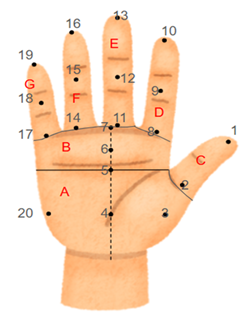
\includegraphics[width=0.4\textwidth]{fig/hand_thickness_points.png}
  \caption{掌測定箇所}
  \label{fig:hand_thickness_points}
\end{figure}

\begin{table}[htbp]
  \centering
  \caption{被験者Aにおける掌領域別厚み測定結果および体積算出例}
  \label{tab:hand_region_thickness}
  \begin{tabular}{c c c c c}
    \hline
    測定箇所 & 厚み (mm) & 平均厚み (mm) & 面積 (cm$^2$) & 体積 (cm$^3$) \\
    \hline
    1  & 16.9  &        &        &        \\
    2  & 18.35 & 17.63  & 15.873 & 27.976 \\
    \hline
    3  & 41.0  &        &        &        \\
    4  & 46.9  &        &        &        \\
    20 & 40.5  & 42.80  & 61.918 & 265.008 \\
    \hline
    5  & 35.025 &        &        &        \\
    6  & 29.8   &        &        &        \\
    7  & 25.07  & 29.97  & 37.673 & 112.886 \\
    \hline
    8  & 19.1  &        &        &        \\
    9  & 14.8  &        &        &        \\
    10 & 13.5  & 15.80  & 14.823 & 23.421 \\
    \hline
    11 & 19.1  &        &        &        \\
    12 & 14.8  &        &        &        \\
    13 & 13.5  & 15.80  & 17.131 & 27.066 \\
    \hline
    14 & 17.0  &        &        &        \\
    15 & 13.5  &        &        &        \\
    16 & 12.0  & 14.17  & 14.451 & 20.472 \\
    \hline
    17 & 14.7  &        &        &        \\
    18 & 12.25 &        &        &        \\
    19 & 10.9  & 12.62  & 11.994 & 15.132 \\
    \hline
    \multicolumn{4}{r}{総体積 (cm$^3$)} & 491.962 \\
    \hline
  \end{tabular}
\end{table}

%--------------------------------------------------

\section{測定結果}

掌面積の測定は、左右それぞれ3回ずつ実施し、
その平均値を各被験者の代表値とした。
複数回測定を行った理由は、
スキャナーの読み取り誤差や
手の置き方によるばらつきを低減し、
再現性および信頼性の高いデータを得るためである。

各被験者の左右の平均掌面積および掌体積を
表\ref{tab:hand_area_volume}に示す。

\begin{table}[htbp]
  \centering
  \caption{被験者ごとの掌面積および掌体積}
  \label{tab:hand_area_volume}
  \begin{tabular}{c|cc|cc}
    \hline
    被験者名 & \multicolumn{2}{c|}{掌の面積 (cm$^2$)} & \multicolumn{2}{c}{掌の体積 (cm$^3$)} \\
             & 右 & 左 & 右 & 左 \\
    \hline
    A & 172.88  & 167.13  & 491.96  & 479.67 \\
    B & 136.88  & 136.75  & 358.86  & 349.48 \\
    C & 134.15  & 138.25  & 338.22  & 335.20 \\
    D & 143.46  & 137.52  & 352.03  & 316.30 \\
    E & 136.88  & 134.00  & 357.28  & 326.40 \\
    F & 153.90  & 148.56  & 306.57  & 311.32 \\
    G & 136.99  & 139.09  & 342.12  & 349.95 \\
    H & 137.88  & 137.81  & 406.86  & 336.94 \\
    I & 135.17  & 129.81  & 256.38  & 223.61 \\
    \hline
  \end{tabular}
\end{table}

%--------------------------------------------------

\section{掌面積および体積の左右差に関する解析結果}

9名の被験者を対象として、
左右の掌面積および体積の差について解析を行った。
解析には対応のある$t$検定を用い、
有意水準は5\%（$p<0.05$）とした。

その結果を表\ref{tab:hand_lr_ttest}に示す。
掌面積では右手が平均でわずかに大きい傾向
（+1.5\%）を示したものの、
統計的に有意な差は認められなかった
（$p=0.127$）。
一方、掌体積では右手が平均で約6.2\%大きく、
統計的に有意な差が認められた
（$p=0.0399$）。

\begin{table}[htbp]
  \centering
  \caption{掌面積および掌体積における左右差の統計解析結果}
  \label{tab:hand_lr_ttest}
  \begin{tabular}{l c c c c c}
    \hline
    項目 & 平均差 & 左右差割合 (\%) & $t$値 & $p$値 & 有意差 \\
    \hline
    掌の面積 & 2.04\,cm$^2$ & 1.50 & 1.70 & 0.127 & なし \\
    掌の体積 & 19.93\,cm$^3$ & 6.20 & 2.45 & 0.0399 & あり \\
    \hline
  \end{tabular}
\end{table}

これらの結果から、
掌面積には有意な左右差は認められなかったが、
掌体積においては利き手側の使用頻度や
筋肉量の発達が反映されている可能性が示唆された。

%--------------------------------------------------

\section{掌面積および体積の左右差に関する考察}

本研究において、掌面積および掌体積の左右差について検討した結果、
掌面積では個人差が大きく、
利き手による影響は統計的に明確ではなかった。
一方で、掌体積においては
右手が有意に大きい結果が得られた。

掌体積に有意な左右差が認められた要因として、
利き手側の使用頻度の高さや
筋肉量の発達が掌の厚みに反映された可能性が考えられる。
日常生活において利き手は非利き手に比べて使用頻度が高く、
把持動作や荷重が繰り返されることから、
筋組織や軟部組織の発達が
掌体積の増加として現れた可能性が高い。

一方、掌面積については
有意な左右差が認められなかった。
掌面積は骨格構造や手の外形に依存する形態的指標であり、
日常的な使用による変化が生じにくいと考えられる。
そのため、利き手・非利き手間においても
統計的に有意な差が
現れなかったものと推察される。

これらの結果は、
利き手優位性（hand dominance）に関する
既存の知見とも整合的であり、
機能的な使用頻度の違いが
厚みや体積といった立体的指標に反映されやすい一方で、
平面的な形状には
反映されにくいことを示唆している。

本研究では被験者数が限られているため、
利き手の影響を十分に一般化するには至らない。
今後は被験者数を増加させるとともに、
利き手情報を明確に取得したうえで解析を行うことで、
利き手と非利き手の
構造的および機能的差異を
より詳細に評価できると考えられる。

%--------------------------------------------------

\section{本章のまとめ}

本章では、後続章におけるウイルス付着実験および洗浄実験に先立ち、
掌面積および体積を定量的に評価する手法を確立した。
これにより、被験者間の身体的差異を考慮した
付着量および残存量の比較が可能となり、
以降の解析およびリスク評価の基盤が整えられた。

% chap3.tex
\chapter{掌表面の付着水分量の測定と\\
\hspace{4\zw}統計解析}

\section{本章の目的}

本章では、掌が水に接触した際にどの程度の水分が皮膚表面に付着・保持されるのかを
定量的に評価することを目的とした。
手指は日常的に外気やさまざまな物体に触れており、その皮膚状態は温度、湿度、
使用環境などの影響を受けやすい。
そのため、同一人物であっても皮膚の厚さやしわの状態、利き手・非利き手といった
使用頻度の違いによって、水分の付着量に差が生じる可能性が考えられる。

本研究では、右手および左手を同一条件下で水に浸漬し、
一定時間保持した後に引き上げる操作を繰り返すことで、
手の形状や皮膚状態の違いが水分付着量に与える影響を評価した。
さらに、測定動作を可能な限り一定化することで、
時間や手の動かし方による誤差を低減し、
掌表面に保持される水分量をより正確に測定することを試みた。

また、被験者間の個人差を評価するため、
身体的特徴の異なる被験者9名を対象として測定を行い、
後続章におけるウイルス付着量および洗浄後残存量の評価に必要な
基礎データを取得することを本章の目的とした。

%--------------------------------------------------

\section{実験材料}

本研究における掌への水分付着量測定には、
以下の器具および材料を使用した。

\begin{itemize}
  \item 蒸留水（900mL）
  \item トレー（水を保持するため）
  \item 電子天秤（質量変化測定用）
  \item 使い捨て紙タオル
\end{itemize}

測定は外部環境の影響を抑えるため、
風の当たらない室内環境において実施した。

%--------------------------------------------------

\section{掌への水分付着量測定方法}

\subsection{実験条件および測定手順}

測定前に、トレーへ蒸留水900mLを注ぎ、
常に同一水量となるよう調整した。
実験は温度および湿度の影響を受けやすいため、
周囲環境を可能な限り一定に保った状態で実施した。

測定前には、被験者に石けんを用いて手を十分に洗浄させ、
使い捨て紙タオルで水分を拭き取った後、測定を開始した。

測定手順を以下に示す。

\begin{enumerate}
  \item 片方の手を用いて測定を行う。
  \item 手を蒸留水中へ静かに挿入し、手全体が水に浸るようにする。
  \item 約5秒間静止させ、掌全体に水分が均一に付着するようにする。
  \item 手を静かに引き上げ、自然に落下する水滴のみを対象とする。
  \item 手を振るなどの動作は行わず、20秒間静止する。
\end{enumerate}

この操作を右手および左手で交互に行い、
各手について同一条件下で複数回の測定を実施した。

\subsection{秤量による付着水量の算出方法}
手から落下する水滴は、
トレー下部に設置した電子天秤により質量変化として測定した。
20秒間静止後に読み取った質量変化を、
掌に付着した水分量とした。

本測定は、学生8名および教員1名の計9名の被験者を対象として実施し、
各被験者について右手および左手それぞれ25回ずつ測定を行った。
その結果、取得された水分付着量データの総数は
$n = 450$（9名 $\times$ 左右2手 $\times$ 25回）である。

得られた質量値は、水の密度を1.0g/mLと仮定し、
体積（mL）として換算した。

なお、測定結果の一例として、
被験者Aにおける右手および左手の水分付着量の平均値および偏差を
表\ref{tab:water_subjectA}に示す。

\begin{table}[htbp]
  \centering
  \caption{被験者Aにおける掌への水分付着量測定結果（平均値および偏差）}
  \label{tab:water_subjectA}
  \begin{tabular}{lcccc}
    \hline
    被験者 &
    右手平均 (mL) &
    右手偏差 (mL) &
    左手平均 (mL) &
    左手偏差 (mL) \\
    \hline
    A & 1.74 & 0.12 & 1.69 & 0.08 \\
    \hline
  \end{tabular}
\end{table}

%--------------------------------------------------

\section{掌面積による水分付着量の正規化}

本研究では、被験者間の掌の大きさの違いを考慮するため、
第2章で求めた掌面積を用いて水分付着量の正規化を行った。
具体的には、測定された水分付着量を掌面積で除することで、
単位面積あたりの水分付着量を算出した。

この正規化により、掌の大きさに依存しない形で
水分付着特性を比較することが可能となる。

%--------------------------------------------------

\section{統計解析方法}

本研究では、掌に付着する水分量について、左右差および被験者間の個人差を同時に評価するため、
混合効果モデルを用いた解析を行った。混合効果モデルは、繰り返し測定や個人差を含むデータ解析に適した統計手法であり、
評価対象となる要因（固定効果）と、測定対象ごとに生じるばらつき（ランダム効果）を同一のモデル内で扱うことができる。
本解析では、左右の掌の別を固定効果とし、被験者ごとの水分付着量の違いをランダム効果としてモデル化した。
これは、皮膚の状態や水切りの癖など、測定や制御が困難な被験者固有の要因による影響を統計的に考慮するためである。

\subsection{解析モデル}
水分付着量（$mL/cm^2$）を目的変数とし、以下の混合効果モデルを構築した。
\begin{itemize}
    \item 固定効果: 手の別（右手、左手）
    \item ランダム効果: 被験者（9名）
\end{itemize}

\subsection{解析結果}

混合効果モデルによる解析結果を以下に示す。

固定効果において、左手を基準とした場合の右手との差（HandRight）は
$2.59 \times 10^{-5}\,\mathrm{mL/cm^2}$ と推定され、その差は極めて小さかった。
また、この左右差に対する検定の結果、$p = 0.707$ となり、
統計的に有意な差は認められなかった。

一方、ランダム効果として設定した被験者間のばらつきには一定の大きさが認められた。
被験者間の標準偏差は約 $0.0010\,\mathrm{mL/cm^2}$、
同一被験者内の測定誤差の標準偏差は約 $0.00073\,\mathrm{mL/cm^2}$ であり、
水分付着量には被験者間の個人差が存在することが示唆された。

以上の結果より、水分付着量は被験者によって異なる傾向がある一方で、
同一被験者内における左右の掌の違いは統計的に有意ではないことが明らかとなった。
すなわち、水分付着量のばらつきは左右差よりも、
被験者固有の要因によって主に規定されていると考えられる。

このことから、掌面積による補正を行った後においても個人差は残存するものの、
左右差の影響は小さく、実質的に無視できる範囲であると判断される。

本解析により、水分付着量の評価において左右を区別して扱う必要性は低いことが示された。
この結果は、以降のウイルス付着量や残存率、
感染リスク評価に関する解析において、
左右の掌を統合して取り扱うことの妥当性を支持するものである。

また、被験者間の個人差が統計的に確認されたことは、
今後のリスク評価において、
水分付着量を単一の値ではなく、
分布として扱う必要性を示唆している。

\subsection{水分付着量データの分布特性}

混合効果モデルの解析結果より、左右の掌における水分付着量に
統計的に有意な差は認められなかったため、
本節では左右および被験者の測定値を統合した
水分付着量データについて分布特性の検討を行った。

統合した水分付着量データに対して正規確率紙（QQプロット）を作成した結果、
図\ref{fig:qq_water_attachment}に示すように、
データ点は概ね直線上に分布しており、
分布形は正規分布から大きく逸脱していないことが確認された。
\begin{figure}[htbp]
  \centering
  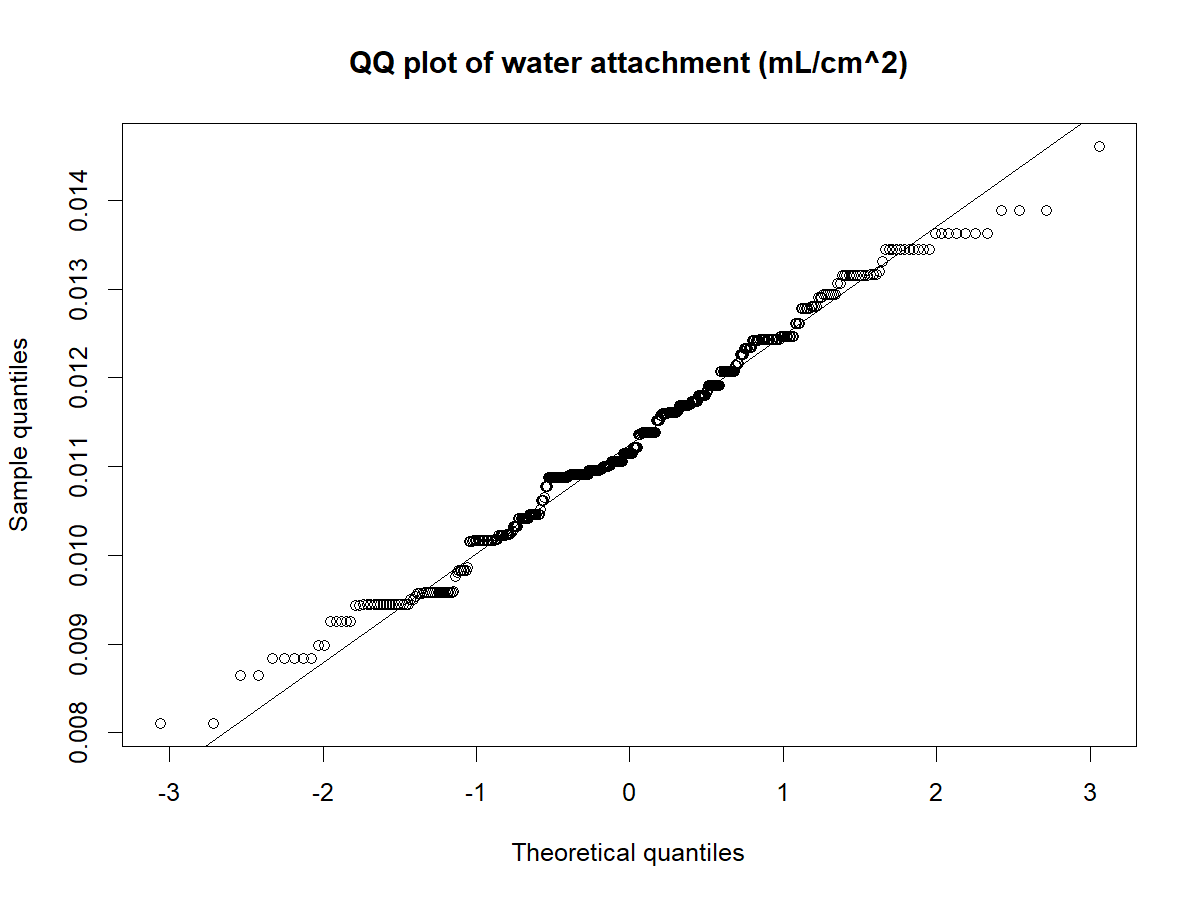
\includegraphics[width=0.7\linewidth]{fig/QQplot_water_attachment.png}
  \caption{水分付着量（mL/cm$^2$）の正規確率紙（QQプロット）}
  \label{fig:qq_water_attachment}
\end{figure}


このことから、
水分付着量（mL/cm$^2$）は、
平均値 $\mu = 0.01128\,\mathrm{mL/cm^2}$、
標準偏差 $\sigma = 0.00119\,\mathrm{mL/cm^2}$ をもつ
正規分布に概ね従うものと判断した。またその分布形を図\ref{fig:hist_water_attachment}に示す。

\begin{figure}[H]
  \centering
  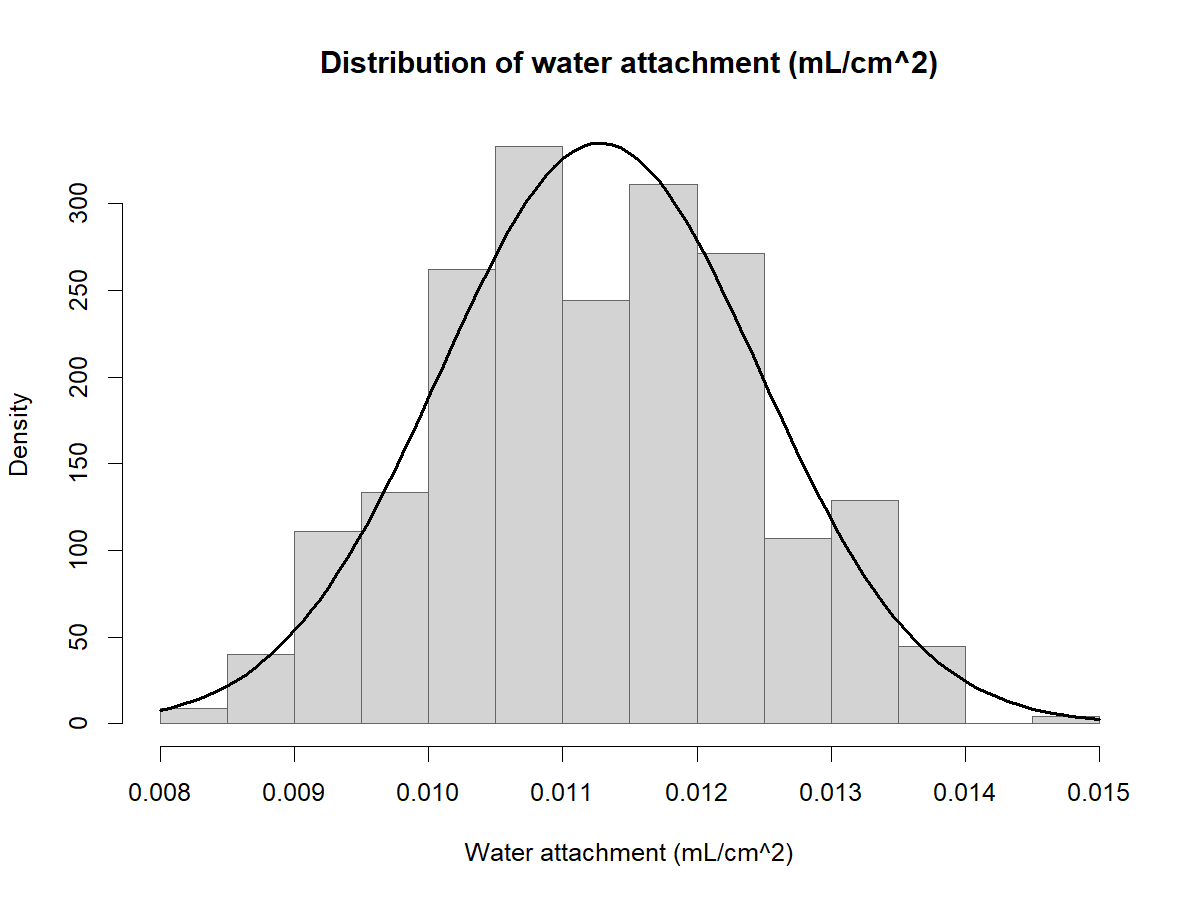
\includegraphics[width=0.7\linewidth]{fig/Histogram_water_attachment_normal.png}
  \caption{%
    水分付着量（mL/cm$^2$）の分布（ヒストグラム）および正規分布曲線\\
    \hspace*{5em}%
    （平均値 $\mu = 0.01128\,\mathrm{mL/cm^2}$，
    標準偏差 $\sigma = 0.00119\,\mathrm{mL/cm^2}$）
  }
  \label{fig:hist_water_attachment}
\end{figure}

%--------------------------------------------------

\section{本章のまとめ}

本章では、掌が水に接触した際の水分付着量を
定量的に測定する手法を確立した。
得られた結果から、水分付着量には
被験者間および左右の手において
一定のばらつきが認められたものの、
全体として大きな個人差は確認されなかった。



\end{document}
